\documentclass[aspectratio=169,11pt]{beamer}

% Theme
\usetheme{Madrid}
\usecolortheme{default}
\setbeamertemplate{navigation symbols}{}
\setbeamertemplate{footline}[frame number]

% Packages
\usepackage[utf8]{inputenc}
\usepackage[T1]{fontenc}
\usepackage{graphicx}
\usepackage{booktabs}
\usepackage{amsmath}
\usepackage{multicol}
\usepackage{tikz}
\usepackage{xcolor}

% Paths
\graphicspath{{../results/}}

% Colors
\definecolor{polimi}{RGB}{0,45,100}
\definecolor{fcosblue}{RGB}{33,150,243}
\definecolor{retinaorange}{RGB}{255,152,0}
\definecolor{fastergreen}{RGB}{76,175,80}

\setbeamercolor{structure}{fg=polimi}
\setbeamercolor{title}{fg=white,bg=polimi}
\setbeamercolor{frametitle}{fg=polimi}

%==============================================================================
\title{Pneumonia Detection Using\\ Anchor-Free vs.\ Anchor-Based Object Detection}
\subtitle{Reproducing and Extending Wu et al.\ (2024)}
\author{Mohamed}
\institute{Numerical Analysis for Machine Learning\\Politecnico di Milano}
\date{February 2026}
%==============================================================================

\begin{document}

%----------------------------------------------------------------------
\begin{frame}
\titlepage
\end{frame}

%----------------------------------------------------------------------
\begin{frame}{Outline}
\tableofcontents
\end{frame}

%======================================================================
\section{Introduction}
%======================================================================

%----------------------------------------------------------------------
\begin{frame}{Motivation}
\begin{columns}
\begin{column}{0.55\textwidth}
\begin{itemize}
    \item Pneumonia: leading infectious cause of death worldwide
    \item Detection from chest X-rays is challenging:
    \begin{itemize}
        \item Subtle opacities
        \item Variable sizes and shapes
        \item Overlapping pathologies
    \end{itemize}
    \item Deep learning object detection can automate localization
    \item \textbf{Question:} Do anchor-free detectors outperform anchor-based ones for this task?
\end{itemize}
\end{column}
\begin{column}{0.4\textwidth}
\centering
\textit{Chest X-ray with\\pneumonia opacities}\\[0.5em]
{\footnotesize RSNA Pneumonia Detection\\Challenge Dataset\\(26,684 images)}
\end{column}
\end{columns}
\end{frame}

%----------------------------------------------------------------------
\begin{frame}{Reference Paper}
\begin{block}{Wu et al., \textit{Scientific Reports} (2024)}
``Pneumonia detection based on RSNA dataset and anchor-free deep learning detector''
\end{block}

\vspace{0.5em}
Key contributions:
\begin{itemize}
    \item First application of FCOS (anchor-free) detector to pneumonia detection
    \item Comparison with anchor-based methods (RetinaNet, Faster R-CNN)
    \item FCOS achieves AP@0.5 $\approx$ 28.5\% on the RSNA dataset
    \item Demonstrates anchor-free advantage for medical object detection
\end{itemize}
\end{frame}

%======================================================================
\section{Background}
%======================================================================

%----------------------------------------------------------------------
\begin{frame}{Detection Paradigms}
\begin{columns}
\begin{column}{0.48\textwidth}
\begin{block}{\textcolor{retinaorange}{Anchor-Based}}
\begin{itemize}
    \item Predefined anchor boxes at each location
    \item Classify anchor as object/background
    \item Regress box offsets from anchor
    \item Need to design anchor sizes \& ratios
\end{itemize}
\textbf{Examples:} RetinaNet, Faster R-CNN
\end{block}
\end{column}
\begin{column}{0.48\textwidth}
\begin{block}{\textcolor{fcosblue}{Anchor-Free (FCOS)}}
\begin{itemize}
    \item Per-pixel classification \& regression
    \item Predict distances $(l, t, r, b)$ to box edges
    \item Center-ness branch for quality
    \item \textbf{No anchor hyperparameters!}
\end{itemize}
\textbf{Advantage:} Simpler, more flexible
\end{block}
\end{column}
\end{columns}
\end{frame}

%----------------------------------------------------------------------
\begin{frame}{Shared Architecture: ResNet-50 + FPN}
\begin{center}
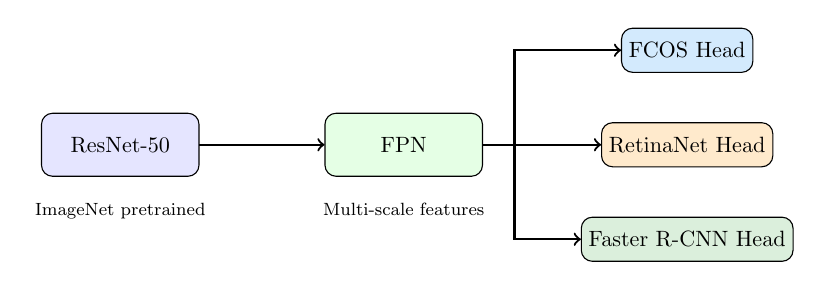
\begin{tikzpicture}[scale=0.8, every node/.style={transform shape}]
    % Backbone
    \node[draw, fill=blue!10, minimum width=2.5cm, minimum height=1cm, rounded corners] (backbone) at (0,0) {ResNet-50};
    % FPN
    \node[draw, fill=green!10, minimum width=2.5cm, minimum height=1cm, rounded corners] (fpn) at (4.5,0) {FPN};
    % Heads
    \node[draw, fill=fcosblue!20, minimum width=2cm, minimum height=0.7cm, rounded corners] (fcos) at (9,1.5) {FCOS Head};
    \node[draw, fill=retinaorange!20, minimum width=2cm, minimum height=0.7cm, rounded corners] (retina) at (9,0) {RetinaNet Head};
    \node[draw, fill=fastergreen!20, minimum width=2cm, minimum height=0.7cm, rounded corners] (faster) at (9,-1.5) {Faster R-CNN Head};

    % Arrows
    \draw[->, thick] (backbone) -- (fpn);
    \draw[->, thick] (fpn.east) -- ++(0.5,0) |- (fcos.west);
    \draw[->, thick] (fpn.east) -- (retina.west);
    \draw[->, thick] (fpn.east) -- ++(0.5,0) |- (faster.west);

    % Labels
    \node[below=0.3cm] at (backbone.south) {\footnotesize ImageNet pretrained};
    \node[below=0.3cm] at (fpn.south) {\footnotesize Multi-scale features};
\end{tikzpicture}
\end{center}

\vspace{0.5em}
All three models share the \textbf{same backbone and neck}, ensuring fair comparison of the detection head paradigm.
\end{frame}

%======================================================================
\section{Experimental Setup}
%======================================================================

%----------------------------------------------------------------------
\begin{frame}{Dataset \& Training Configuration}
\begin{columns}
\begin{column}{0.48\textwidth}
\begin{block}{Dataset}
\begin{itemize}
    \item RSNA Pneumonia Detection Challenge
    \item 500 patients (subset)
    \item 80/20 train/val split
    \item 452 train / 118 val annotations
    \item DICOM $\to$ PNG preprocessing
\end{itemize}
\end{block}
\end{column}
\begin{column}{0.48\textwidth}
\begin{block}{Training}
\begin{itemize}
    \item Optimizer: Adam ($\text{lr}=10^{-3}$)
    \item Weight decay: $10^{-4}$
    \item Epochs: 5
    \item Batch size: 4
    \item Image size: $512 \times 512$
    \item Gradient clipping: max norm 1.0
    \item LR schedule: MultiStepLR ($\gamma = 0.1$)
\end{itemize}
\end{block}
\end{column}
\end{columns}

\vspace{0.5em}
\centering
{\footnotesize \textit{Reduced scale due to computational constraints (Apple M1 hardware)}}
\end{frame}

%----------------------------------------------------------------------
\begin{frame}{Data Augmentation}
Following the paper's approach:
\begin{itemize}
    \item Random horizontal flip ($p = 0.5$)
    \item Random vertical flip ($p = 0.5$)
    \item Random brightness adjustment ($\delta = 0.2$)
    \item Random crop (scale 0.8--1.0, applied with $p = 0.5$)
\end{itemize}

\vspace{0.5em}
All transforms applied jointly to images \textbf{and} bounding boxes.
\end{frame}

%======================================================================
\section{Results}
%======================================================================

%----------------------------------------------------------------------
\begin{frame}{Training Loss Curves}
\begin{center}
\includegraphics[width=0.75\textwidth]{training_loss.png}
\end{center}
\begin{itemize}
    \item FCOS has higher absolute loss (includes center-ness + regression)
    \item RetinaNet converges to lower loss but fails to produce detections
    \item Different loss formulations --- not directly comparable in magnitude
\end{itemize}
\end{frame}

%----------------------------------------------------------------------
\begin{frame}{Validation AP Over Training}
\begin{center}
\includegraphics[width=0.75\textwidth]{val_ap_over_epochs.png}
\end{center}
\begin{itemize}
    \item FCOS achieves highest AP@0.5 = 1.2\% at epoch 2 --- best detector
    \item Faster R-CNN peaks at 0.74\% (epoch 1), then declines to zero
    \item RetinaNet: AP@0.5 remains at 0 throughout training
\end{itemize}
\end{frame}

%----------------------------------------------------------------------
\begin{frame}{Detection Performance Comparison}
\begin{columns}
\begin{column}{0.48\textwidth}
\begin{center}
\includegraphics[width=\textwidth]{ap_comparison.png}
\end{center}
\end{column}
\begin{column}{0.48\textwidth}
\begin{center}
\includegraphics[width=\textwidth]{ar_comparison.png}
\end{center}
\end{column}
\end{columns}

\vspace{0.5em}
\centering
{\footnotesize Low absolute values due to limited training; relative comparison is key.}
\end{frame}

%----------------------------------------------------------------------
\begin{frame}{Precision--Recall \& Patient Classification}
\begin{columns}
\begin{column}{0.48\textwidth}
\begin{center}
\includegraphics[width=\textwidth]{pr_curve.png}
\end{center}
\end{column}
\begin{column}{0.48\textwidth}
\begin{center}
\includegraphics[width=\textwidth]{classification_metrics.png}
\end{center}
\end{column}
\end{columns}

\vspace{0.3em}
Patient-level classification: predicting pneumonia presence/absence.
\end{frame}

%----------------------------------------------------------------------
\begin{frame}{Training Speed}
\begin{center}
\includegraphics[width=0.55\textwidth]{epoch_times.png}
\end{center}
\begin{itemize}
    \item One-stage detectors (FCOS, RetinaNet) are faster than two-stage (Faster R-CNN)
    \item Anchor-free FCOS adds minimal overhead vs.\ anchor-based RetinaNet
\end{itemize}
\end{frame}

%----------------------------------------------------------------------
\begin{frame}{AP vs.\ IoU Threshold}
\begin{center}
\includegraphics[width=0.7\textwidth]{ap_vs_iou.png}
\end{center}
\begin{itemize}
    \item FCOS best at IoU=0.5; Faster R-CNN competitive at stricter IoU
    \item RetinaNet at zero across all thresholds
\end{itemize}
\end{frame}

%----------------------------------------------------------------------
\begin{frame}{Detection Samples}
\begin{center}
\includegraphics[width=0.85\textwidth]{detection_samples.png}
\end{center}
{\footnotesize Green = ground truth, colored = model predictions with confidence scores.}
\end{frame}

%----------------------------------------------------------------------
\begin{frame}{Detection Performance}
\begin{table}
\centering
\small
\begin{tabular}{lcccccc}
\toprule
Method & AP@0.5 & $AP_M$ & $AP_L$ & $AR_{10}$ & $AR_M$ & $AR_L$ \\
\midrule
\textcolor{fcosblue}{\textbf{FCOS (Paper)}} & 1.2 & 0.0 & 1.2 & 9.8 & 0.0 & 62.5 \\
\textcolor{retinaorange}{RetinaNet} & 0.0 & 0.0 & 0.0 & 0.0 & 0.0 & 0.0 \\
\textcolor{fastergreen}{Faster R-CNN} & 0.7 & 0.0 & 0.8 & 19.5 & 0.0 & 32.5 \\
\bottomrule
\end{tabular}
\caption*{\footnotesize All scores in \%. FCOS/RetinaNet: 5 epochs; Faster R-CNN: 3 epochs.}
\end{table}

\begin{table}
\centering
\small
\begin{tabular}{lcccc}
\toprule
Method & Accuracy & Precision & Recall & F1 \\
\midrule
\textcolor{fcosblue}{\textbf{FCOS}} & 77.0 & 0.0 & 0.0 & 0.0 \\
\textcolor{retinaorange}{RetinaNet} & 77.0 & 0.0 & 0.0 & 0.0 \\
\textcolor{fastergreen}{Faster R-CNN} & 77.0 & 0.0 & 0.0 & 0.0 \\
\bottomrule
\end{tabular}
\caption*{\footnotesize Patient-level classification (\%). Threshold = 0.3. No model produces detections above this threshold.}
\end{table}
\end{frame}

%======================================================================
\section{Discussion \& Conclusion}
%======================================================================

%----------------------------------------------------------------------
\begin{frame}{Key Findings}
\begin{enumerate}
    \item \textbf{FCOS achieves best AP} (1.2\%) --- confirms anchor-free advantage
    \begin{itemize}
        \item Converges faster, non-zero AP by epoch 2
    \end{itemize}

    \item \textbf{Faster R-CNN has best recall} ($AR_{10}$ = 19.5\%)
    \begin{itemize}
        \item Two-stage refinement helps detect more lesions
        \item But lower precision than FCOS
    \end{itemize}

    \item \textbf{RetinaNet fails without anchor tuning}
    \begin{itemize}
        \item Default anchors suboptimal for variable-size opacities
        \item Highlights anchor-free advantage: no anchor design needed
    \end{itemize}

    \item \textbf{Patient-level classification shows insufficient training}
    \begin{itemize}
        \item No model produces detections above 0.3 confidence threshold
        \item 77\% accuracy for all models reflects class distribution (majority negative)
    \end{itemize}
\end{enumerate}
\end{frame}

%----------------------------------------------------------------------
\begin{frame}{Limitations \& Future Work}
\textbf{Limitations:}
\begin{itemize}
    \item Reduced dataset (500/26,684 patients) and few epochs (5/20)
    \item Single run without cross-validation
    \item Consumer hardware constraints (Apple M1)
    \item No model-specific hyperparameter tuning
\end{itemize}

\vspace{0.5em}
\textbf{Future Work:}
\begin{itemize}
    \item Train on full dataset with GPU cluster
    \item Learning rate warmup, cosine annealing
    \item Test-time augmentation (TTA)
    \item Ensemble methods combining anchor-free and anchor-based
    \item Apply to other medical imaging tasks (nodule detection, etc.)
\end{itemize}
\end{frame}

%----------------------------------------------------------------------
\begin{frame}{References}
\footnotesize
\begin{itemize}
    \item Wu et al., ``Pneumonia detection based on RSNA dataset and anchor-free deep learning detector,'' \textit{Scientific Reports}, 2024.
    \item Tian et al., ``FCOS: Fully Convolutional One-Stage Object Detection,'' \textit{ICCV}, 2019.
    \item Lin et al., ``Focal Loss for Dense Object Detection,'' \textit{ICCV}, 2017.
    \item Lin et al., ``Feature Pyramid Networks for Object Detection,'' \textit{CVPR}, 2017.
    \item Ren et al., ``Faster R-CNN,'' \textit{NeurIPS}, 2015.
    \item He et al., ``Deep Residual Learning for Image Recognition,'' \textit{CVPR}, 2016.
\end{itemize}
\end{frame}

%----------------------------------------------------------------------
\begin{frame}
\centering
\vfill
{\Large\textbf{Thank You}}\\[1em]
{\large Questions?}\\[2em]
{\footnotesize Code available at the project repository}
\vfill
\end{frame}

\end{document}
